\section{FastAD Implementation}\label{sec:fastad}

In this section, we cover a few key ideas of our implementation\footnotemark.
\footnotetext{github page: https://github.com/JamesYang007/FastAD}
In Section~\ref{ssec:vectorization},
we first discuss the benefits of vectorization and the difficulties of integrating it into an AD system.
We then explain how FastAD fully utilizes vectorization
and demonstrate that other libraries do not fully take advantage of it. 
In Section~\ref{ssec:memory},
we discuss some memory management and performance issues
stemming from the use of the ``tape'' data structure.
We then explain how FastAD overcomes these challenges using expression templates
and a lazy allocation strategy.\@
Finally, Section~\ref{ssec:compile-time-opt} covers other compile-time optimizations 
that can further maximize performance.

\subsection{Vectorization}\label{ssec:vectorization}

Vectorization refers to the parallelization of operations on multiple data at the hardware level.
On a modern Intel 64-bit processor supporting AVX, 
four double-precision floating point numbers can be processed simultaneously,
roughly improving performance by a factor of four.
While the compiler optimization is able to vectorize a user's code sometimes, it is not guaranteed
because vectorization requirements are quite stringent. 
For example, vectorization is not guaranteed if memory access is not done in a contiguous fashion
and is impossible if there is any dependency between loop iterations.
This makes it quite challenging to design an AD system that 
can always predict compiler optimization to create vectorized code.
However, vectorization can make AD extremely fast, powerful, and practical even in complex problems.
In practice, we come across many examples where operations can be vectorized during gradient computation.
For example, matrix multiplication, any reduction from a multi-dimensional variable to a scalar such as
summation or product of all elements, and any unary and binary function that is applied element-wise such as
exponential, logarithm, power, sin, cos, tan, and the usual arithmetic operators.

Since most of the opportunities for vectorization occur in matrix operations,
the goal is to use a well-polished and efficient
matrix library such as \code{Eigen}, one of the most popular C++ matrix libraries.
However, this is not an easy task.
Adept2.0 notes in their documentation that integrating an expression-template based matrix library 
such as \code{Eigen} into an AD system can be quite challenging in design.
To circumvent these design issues, 
Adept2.0 integrates their own matrix library designed specifically for their AD system.
This, however, only introduces another problem of writing an efficient matrix library, another daunting task.
In fact, the author of Adept notes that matrix multiplication,
one of the most widely used matrix operations, 
is currently very slow~\cite{hogan:2014}.
Stan mentions that integrating matrix libraries can lead to unexpected problems 
that would require extra memory allocations to resolve~\cite{carpenter:2015}.
Other libraries such as ADOL-C, CppAD, and Sacado do not integrate any matrix libraries directly,
but they do allow the use of \code{Eigen} matrix classes simply as containers.

The one library among those mentioned previously that ultimately incorporates \code{Eigen} is Stan.
Stan provides their own ``plug-ins'', which extend \code{Eigen} classes for their AD variables.
For example, in Stan, one would use \\
\code{Eigen::Matrix<stan::math::var, \ldots>} as a matrix of AD (univariate) variables,
where the generic matrix object is extended to work differently for \code{stan::math::var}.
However, this design still does not take full advantage of the vectorization that \code{Eigen} provides.
One reason is that \code{Eigen} is only highly optimized for matrices of primitive types such as double-precision floating points and integers.
For any other class types, \code{Eigen} defaults to a less optimized version with no guarantees of vectorization.
Therefore, unless one extends all \code{Eigen} methods with optimizations for their specific class type,
they will not receive much benefit of vectorization.
Another reason is that these matrices now have a heterogeneous structure where
each element is an AD variable which represents a pair of value and adjoint.
As a result, it is not possible to read only the values (and similarly, only the adjoints) of the matrix in a contiguous fashion.
The compiler then cannot guarantee any automatic vectorization.

\begin{figure*}[t]
    \centering
    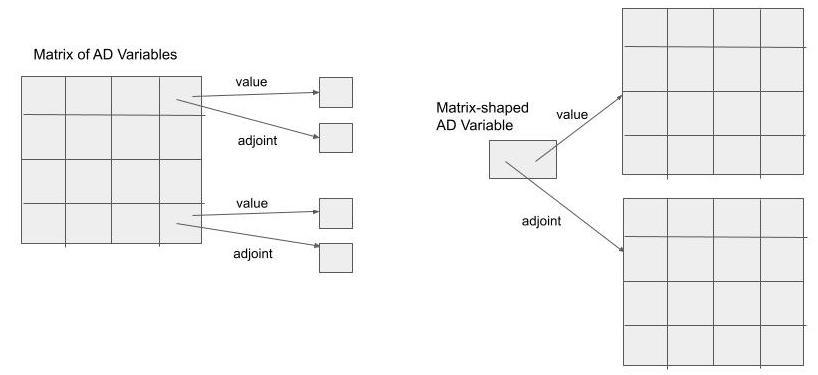
\includegraphics[width=0.8\textwidth]{fastad/figs/matrix-memory-layout.jpg}
    \caption{%
        The left shows the memory layout for a matrix of univariate AD variables.
        This refers to the design pattern ``a matrix of pair of pointers to double''
        since each element of the matrix contains two pointers pointing to its value and adjoint.
        The right shows the memory layout for a single matrix-shaped AD variable,
        referring to the reverse pattern ``a pair of pointers to matrix of doubles''.
        This AD variable has two pointers, each pointing to a matrix of doubles for the value and adjoint.
    }\label{fig:matrix-memory-layout}
\end{figure*}

FastAD fully utilizes the benefits of \code{Eigen} through one simple design difference, which we refer to as \emph{shape traits}.
Stan as well as the other libraries mentioned previously except Adept2.0
follow the design pattern of ``a matrix of pair of pointers to double'' when defining a matrix of AD variables.
Note that a univariate AD variable internally contains two pointers to doubles,
one pointing to the value and one to the adjoint.
In contrast, FastAD follows the reverse pattern: ``a pair of pointers to matrix of doubles''.
That is, rather than defining a univariate AD variable, which gets reused as an element of a matrix,
we define a separate matrix AD variable containing a pair of pointers, each pointing to a matrix of double.
Figure~\ref{fig:matrix-memory-layout} shows the memory layout for each of the design patterns.
This subtle difference provides a few important benefits.
Since the value and adjoint are now represented as matrices of primitive types,
matrix operations will be vectorized.
The second benefit is the significant reduction of memory consumption.
For other libraries, a matrix of AD variables contains two pointers \emph{for each element}.
However, with our design, a single matrix AD variable would only store two pointers
regardless of the size of the matrix.
Hence, if a matrix is $m\times n$, 
the traditional approach has a $O(mn)$ memory consumption for the pointers,
and FastAD approach has a $O(1)$ consumption.

Using templates in C++,
it is easy to unify the API for the different AD variable shapes
by providing an additional template parameter:
\begin{lstlisting}[style=customcpp]
ad::Var<double, ad::scl> x; // scalar shape
ad::Var<double, ad::vec> v; // vector shape
ad::Var<double, ad::mat> m; // matrix shape
\end{lstlisting}

Shape traits also apply for any arbitrary node because
we can deduce the output shape given the input shapes.
The following is a declaration of a generic node representing an
element-wise unary operation, which demonstrates this idea:
\begin{lstlisting}[style=customcpp]
template <class Unary, class ExprType>
struct UnaryNode:
    ValueAdjView<
      typename util::expr_traits<ExprType>::value_t,
      <@\textcolor{red}{typename util::shape\_traits<ExprType>::shape\_t}@>>
{ /*...*/ };
\end{lstlisting}
The portion highlighted in red related to \code{shape\_t}
takes the input expression type \code{ExprType} and deduces its shape type.
Since an element-wise unary operation always has the same shape as its input,
the unary node takes on the same shape.

To verify that FastAD vectorizes more than Stan, 
we performed reverse-AD for a simple summation function $f(x) = \sum\limits_{i=1}^n x_i$
and generated the disassembly for Stan and FastAD~\footnotemark.\@
\footnotetext{github page: https://github.com/JamesYang007/ADBenchmark}
We extracted the part that performs the summation
and compared the instructions to see whether vectorization was taking place.\@
The following is the disassembly for Stan:
\begin{lstlisting}[style=customasm]
L3178:
    movq    (%rax), %rdx
    addq    $8, %rax
    <@\textcolor{red}{vaddsd}@>   8(%rdx), %xmm0, %xmm0 
    cmpq    %rcx, %rax 
    jne L3178
\end{lstlisting}
The instruction used to add is \code{vaddsd},
which is an AVX instruction to add \emph{scalar} double-precision values.
This is not a vectorized instruction, and hence the addition is not done in parallel.
This portion of the disassembly is related to a specialization of an \code{Eigen} class 
responsible for summation with \emph{default traversal},
which is no different from a naive for-loop.

Compare the above disassembly with the one generated for FastAD:
\begin{lstlisting}[style=customasm]
 L3020:
     addq    $8, %rdx
     <@\textcolor{red}{vaddpd}@>  (%rax), %ymm1, %ymm1   
     <@\textcolor{red}{vaddpd}@>  32(%rax), %ymm0, %ymm0 
     addq    $64, %rax
     cmpq    %rdx, %rcx 
     jg  L3020 
\end{lstlisting}
This portion of the assembly is indeed related to the \emph{linear vectorized traversal}
specialization of the same \code{Eigen} class responsible for the summation.
The instruction used to add is \code{vaddpd},
which is an AVX instruction to add \emph{packed} double-precision values.
This is a vectorized instruction and the operation is truly done in parallel.

Sometimes, Stan is able to produce vectorized code such as in matrix multiplication.
This is consistent with our benchmark results 
since Stan came closest to FastAD for this operation (see Section~\ref{ssec:matrix_mult}).
It is also consistent with how it is implemented,
since they allocate extra memory for \code{double} values for each matrix 
and the multiplication is carried out with these matrices of primitive types.
However, this vectorization does come at a cost of at least 4 times extra memory allocation than what FastAD allocates.
Moreover, the backward-evaluation requires heap-allocating a matrix on-the-fly every time.
FastAD incurs no such cost, only allocates what is needed, and never heap-allocates during AD evaluation.


\subsection{Memory Management}\label{ssec:memory}

Most AD systems manage a data structure in memory often referred to as the ``tape''
to store the sequence of operations via function pointers as well as the node values and adjoints.
This tape is modified dynamically and requires sophisticated memory management 
to efficiently reuse memory whenever possible.
Stan even writes their own custom memory allocator to alleviate memory fragmentation,
promote data locality, and amortize the cost of memory allocations~\cite{carpenter:2015}.
However, the memory is not fully contiguous and may still over-allocate.
For some libraries, on top of memory management of these operations,
a run-time check must be performed at every evaluation to determine the correct operation~\cite{bell:2020}.
Others like Stan rely on dynamic polymorphism to look up the vtable to call the correct operation~\cite{carpenter:2015}.

FastAD is unique in that it uses expression templates to represent the sequence of operations
as a single stack-allocated object.
By overloading the comma operator, we can chain expressions together into a single object.
The following is an example of chaining multiple expressions:
\begin{lstlisting}[style=customcpp]
auto expr = (
    x = y * z,                      // expr 1
    w = x * x + 3 * ad::sin(x + y), // expr 2
    w + z * x                       // expr 3
);
\end{lstlisting}
Each of the three sub-expressions separated by the commas returns an expression object
containing the necessary information to perform reverse-AD on their respective structure.
Those expression objects are then chained by the comma operators to build a final expression object
that contains the information to perform reverse-AD on all 3 sub-expressions in the order presented.
This final object is saved into the variable \code{expr}.

Expression template makes it possible to build these expression objects containing the reverse-AD logic.
Expression template is a template metaprogramming technique that builds complex
structures representing a computation at compile-time.
For a full treatment of expression templates, we direct the readers to~\cite{vandevoorde:2002}.
As an example, in the following case,
\begin{lstlisting}[style=customcpp]
Var<double, scl> x, y;
auto expr = x + y;
\end{lstlisting}
\code{x+y} returns a new object of type
\code{BinaryNode<Add, Var<double, scl>, Var<double, scl>>},
which represents the addition of two AD variables.
In particular, this object has member functions that define the logic for
the forward and backward evaluations of the reverse-mode AD.\@
This design brings many performance benefits.
Since the compiler now knows the entire sequence of operations for the expression,
it allows for the reverse-AD logic to be inlined with no virtual function calls,
and it removes the need to dynamically manage a separate vector of function pointers.
Additionally, the expression object is stack-allocated,
which is cheaper than being heap-allocated,
and its byte size is proportional to the number of nodes,
which is relatively small in practice.

We can optimize the memory management even further with another observation:
an expression can determine the \emph{exact} number of values and adjoints needed to represent all of the nodes.
If every node can determine this number for itself,
then any expression tree built using these nodes can determine it as well by induction.
It is the case that all nodes defined in FastAD can, in fact, determine this number.
This leads to the idea of \emph{lazy allocation}.
Lazy allocation refers to allocating memory only when the memory is required by the user.
In other words, an expression object does not necessarily need to 
allocate memory for the values and adjoints at construction time,
since it is only needed later at differentiation time.
Once an expression is fully built and the user is ready to differentiate it,
the user can lazily determine this number of values and adjoints by interfacing with the expression object,
allocate that amount in a contiguous manner,
and ``bind'' the expression object to use that region of memory.
This solves the issue with the traditional tape where the values and adjoints are
not stored in a fully contiguous manner.
Conveniently, the allocated values and adjoints also do not necessarily 
need to be stored and managed by a global tape.
Furthermore, the expression objects can be given additional logic 
to bind to this region systematically so that the forward and backward evaluations
will read this memory region almost linearly, which increases cache hits.

While Stan notes that they are more memory-efficient than other popular C++ libraries~\cite{carpenter:2015},
we noticed a non-negligible difference in memory consumption between Stan and FastAD.
We took the stochastic volatility example in Section~\ref{ssec:stochastic_volatility},
and compared the memory allocation in number of bytes.
For Stan, we took the member variables
from the tape and computed the number of used bytes.
We did not take into account other miscellaneous members for simplicity,
and this estimate serves as a very rough lower bound on the total amount of memory allocated.
For FastAD, we computed the memory allocated for the values, adjoints, and the expression object.
Our result shows that Stan uses 4718696 bytes and FastAD uses 1836216 bytes.
This rough estimate shows that Stan uses at least 2.5 times more memory than FastAD.

With all these optimizations, FastAD removes the need for a global tape by 
using expression templates to manage the sequence of operations in an expression at compile-time,
contiguously allocating the exact number of values and adjoints,
and localizing the memory allocations for each expression.


\subsection{Other Compile-Time Optimizations}\label{ssec:compile-time-opt}

Using C++17 features, we can make further compile-time optimizations
that could potentially save tremendous amount of time during run-time.

% choose correct specialization depending on shapes

One example is choosing the correct specialization of an operation
depending on the shapes of the input.
As seen in Section~\ref{ssec:vectorization}, all nodes are given a shape trait.
Depending on the input shapes, one may need to invoke different routines for the same node.
For example, the normal log-pdf node behaves quite differently
depending on whether the variance parameter is a scalar $\sigma^2$
or a (covariance) matrix $\Sigma$.
Namely, if the variance has a matrix shape,
we must perform a matrix inverse to compute the log-pdf,
which requires a different code from the scalar case.
Using a C++ design pattern called Substitution-Failure-Is-Not-An-Error (SFINAE),
we can choose the correct routine at compile-time.
The benefit is that there is no time spent during run-time in choosing the routine anymore,
whereas in libraries like CppAD, they choose the routines at run-time 
\emph{for every evaluation} of the node~\cite{bell:2020}.

% sufficient statistic

Another example is detecting constants in an expression. 
We can optimize a node by saving temporary results when certain inputs are constants,
which we can check at compile-time using the C++ language feature \code{if constexpr}.
These results can then be reused in subsequent AD evaluations,
sometimes changing orders of magnitude of the performance.
As an example, consider an expression containing a normal log-pdf node for which we differentiate many times.
Suppose also that the input variables to the node are $x$, an $n$-dimensional vector of constants,
and $\mu, \sigma$, which are scalar AD variables.
In general, for every evaluation of the node, the time to forward-evaluate the log-pdf is $O(n)$,
since we must compute 
\begin{align*}
    \log(p(x|\mu, \sigma)) &= -\frac{\sum\limits_{i=1}^n (x_i-\mu)^2}{2\sigma^2} - n\log(\sigma) + C
\end{align*}
However, the normal log-pdf node has an opportunity to make a powerful optimization in this particular case.
Since the normal family defines a two-dimensional exponential family,
it admits a sufficient statistic $T(x) = \paren{\bar{x}, S^2_n(x)}$ where
\begin{align*}
    \bar{x} := \frac{1}{n} \sum\limits_{i=1}^n x_i, \,
    S_n^2(x) := \frac{1}{n} \sum\limits_{i=1}^n (x_i - \bar{x})^2
\end{align*}
Since $x$ is a constant, the sufficient statistic can then be computed \emph{once} and saved for future use.
The normal log-pdf forward-evaluation now only takes $O(1)$ time given the sufficient statistic,
as seen in Eq.~\ref{eq:normal_log_pdf_x_const} below,
\begin{align}
    \log(p(x|\mu, \sigma)) 
    &= -\frac{1}{2 \sigma^2} 
        \sum\limits_{i=1}^n (x_i - \mu)^2 
        - n\log(\sigma) + C \nonumber \\
    &= -\frac{n}{2 \sigma^2} 
        \paren{S_n^2 + (\bar{x} - \mu)^2} 
        - n\log(\sigma) + C 
        \label{eq:normal_log_pdf_x_const}
\end{align}

